\documentclass{beamer}\usepackage{graphicx, color}
%% maxwidth is the original width if it is less than linewidth
%% otherwise use linewidth (to make sure the graphics do not exceed the margin)
\makeatletter


\usetheme{Madrid}
%\hypersetup{pdfpagemode=FullScreen}

\setbeamertemplate{footline}[text line]{} % makes the footer EMPTY
\useoutertheme[subsection=false]{smoothbars}

\usepackage{graphicx}
\usepackage{amsthm}


\begin{document}





\begin{frame}
\LARGE
Version Control and Reproducible Research with GitHub \\
\begin{center}
\vspace{2cm}
Tad Dallas \\
December 2013 \\
\end{center}

\includegraphics[width=0.2\textwidth]{ceesglogo.png}
\hfill 
\includegraphics[width=0.2\textwidth]{github-logo.png}
\end{frame}



\begin{frame}
 \frametitle{What is GitHub?}

Code sharing, publishing and development service for collaborative projects

\begin{exampleblock}{Why use it?}
 \begin{itemize}
  \item Version control 
  \item Open collaboration with other scientists
  \item Creepily watch what other people are working on!
 \end{itemize}
\end{exampleblock}

\pause
\begin{block}{Under the hood}
 \begin{itemize}
  \item Git is the version control language that GitHub is the GUI for
  \item Created by Linus Torvalds, a central developer of the Linux OS 
  \item Command-line, but really straight-forward
 \end{itemize}
\end{block}
\end{frame}


\begin{frame}
 \frametitle{A couple quick definitions}
  \begin{itemize}
    \item \textbf{Repository}: Storage space where your projects reside
    \item \textbf{Commit}: Takes 'snapshot' of your repository, so you can log a new change, or revert to a previous state (Common command)
    \item \textbf{Branch}: Think of a folder within a repository, but cooler. More on this later
    \item \textbf{Fork}: What it sounds like. You're taking someone's project and making a copy of it for your own use (either to collaborate and to merge later or to use as a template for a different project)
    \item \textbf{Push}: The act of updating your project files (you will ``push'' your \textbf{commits})
    \item \textbf{Pull}: Gets commits from a repository to your machine
    \item \textbf{Fetch}: A better version of \textbf{pull} that doesn't merge \textbf{commits}
  \end{itemize}
  \end{frame}




\begin{frame}
 \frametitle{How to begin}
\begin{enumerate}
 \item Set up an account (go to https://github.com/) and download Git (http://git-scm.com/downloads)
 \item Open a terminal window
\pause
\begin{center}
 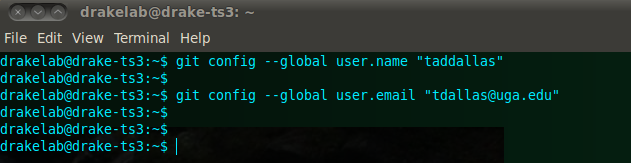
\includegraphics[width=0.85\textwidth]{config.png}
\end{center}
\end{enumerate}
Okay. Now we have Git on our machines and GitHub accounts.
\end{frame}




\begin{frame}
 \frametitle{The GitHub framework}
\begin{block}{Getting your files on GitHub}
\begin{itemize}
 \item Do work in a local directory
 \item Create a Git repo in this local directory 
 \item \textbf{Add} and \textbf{commit} your files ('put stones in the catapult')
 \item \textbf{Push} your files to Github ('catapult those stones')
\end{itemize}
\end{block}


\end{frame}


\begin{frame}
 \frametitle{\textbf{Make your directory}}
% 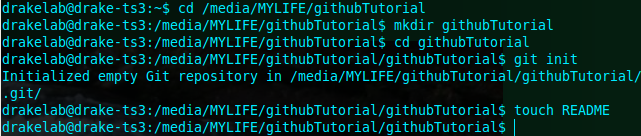
\includegraphics[width=\textwidth]{mkdir.png}\\
\textbf{Sets up local directory} \\
\begin{quote}
  \$ cd \textit{folder you want your directory in} \\
\$ mkdir \textit{directory name} \\
\$ cd \textit{your project directory} \\
\end{quote}

\textbf{Initializes git in that directory}
\begin{quote}
 \$ git init
\end{quote}
Do some stuff in the directory!
\end{frame}



\begin{frame}
\frametitle{\textbf{Committing changes}}
  From within your local directory
  \begin{quote}
    \$ git remote add origin https://github.com/yourname/yourproject.git \\
    \$ git commit -a -m ``message associated with your commit''
  \end{quote}
  \pause
  Only need to do the \textbf{git remote add} command once. You can check to see what your remote locations are by typing \begin{quote}
                                                                                                                           git remote -v
                                                                                                                          \end{quote}
from within your local directory. 
% 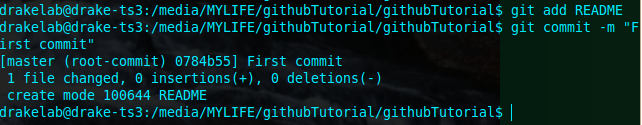
\includegraphics[width=\textwidth]{add.png}\\
\end{frame}


\begin{frame}
\frametitle{\textbf{Push it!}}
 \begin{quote}
  \$ git push origin master
 \end{quote}

% 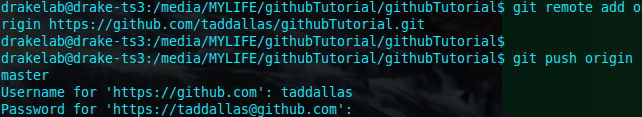
\includegraphics[width=\textwidth]{push.png}\\
\end{frame}



\begin{frame}
 \frametitle{General framework for edits thereafter}
\begin{block}{}
 \begin{enumerate}
  \item Edit your files locally
  %\item \$ git add *files in your local directory*
  \item \$ git commit -a -m ``message about this commit''
  \item \$ git push origin master 
 \end{enumerate}
\end{block}
\end{frame}


\begin{frame}
\frametitle{How to collaborate using GitHub}
Up to this point, it's been a solitary experience of \textbf{making} and \textbf{pushing} \\
 \begin{block}{Methods of collaboration}
Two ways:
\begin{itemize}
 \item \textbf{'Fork and Pull' model} : better
 \item \textbf{'Shared Repository' model} : easier
\end{itemize}
\end{block}


\begin{alertblock}{Pulling files from GitHub}
 \begin{itemize}
  \item cd to local repository
  \item \$ git remote -v  \ \ \  outputs the .git repos you can push/pull to/from. Use \$ git remote add 'http://github.com/name/project.git' if necessary
  \item \$ git pull . \ \ \ fetches and merges files
 \end{itemize}
\end{alertblock}
\end{frame}





%\begin{frame}
% \frametitle{Forking a repo \textit{from} GitHub}
% 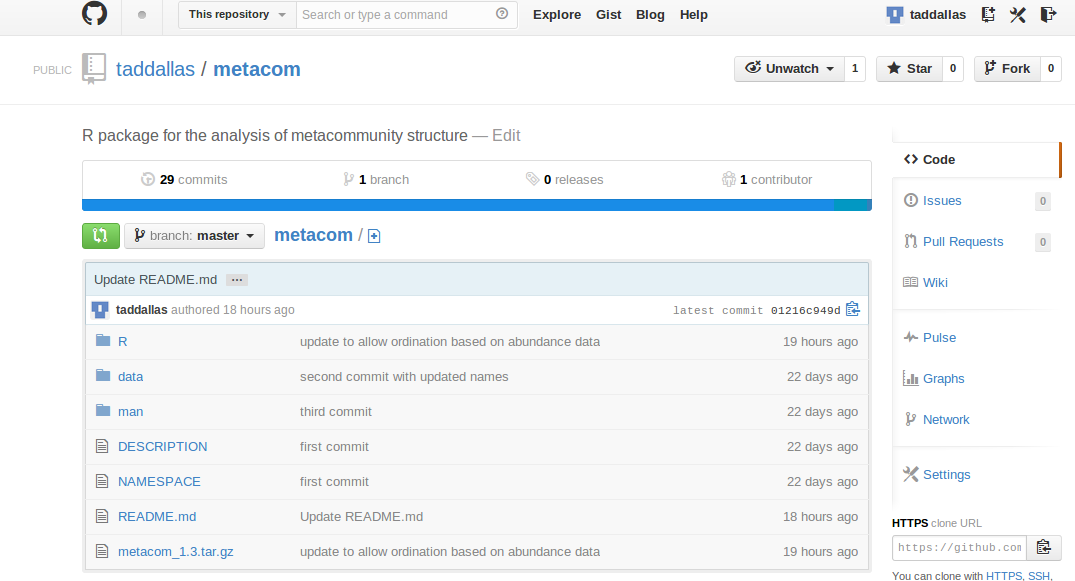
\includegraphics[width=\textwidth]{fork.png}\\
%\end{frame}

\begin{frame}
 \frametitle{Forking from command-line}

 \$ git clone git://github.com/somename/someproject.git someproject \\
\vspace{1cm}
\#This initializes a new local directory on your machine in a folder called 'someproject' \\

\end{frame}


\begin{frame}
 \frametitle{Some useful commands}

\textbf{Check status} : \\ \$ git status \vspace{0.5cm}

\textbf{See your remote locations} : \\ \$ git remote -v \vspace{0.5cm}

\textbf{View commit history} : \\ \$ git log \vspace{0.5cm}

\textbf{Revert to previous version since last commit}:  \\ \$ git checkout -- \textit{filename}

\textbf{See a log of all changes}: \\ \$git log 

\end{frame}




\begin{frame}
\huge Questions?  \\
\vspace{1cm}
\pause
\normalsize Let's now look at the user interface of GitHub and play around a bit 
\end{frame}












\end{document}
